\documentclass[oneside, 11pt]{article}

\usepackage[T1]{fontenc}
\usepackage[utf8]{inputenc}
\usepackage[english]{babel}

\usepackage{fouriernc}
\usepackage[detect-all, binary-units, separate-uncertainty=true,
            per-mode=symbol, retain-explicit-plus, retain-unity-mantissa=false]{siunitx}

\usepackage{setspace}
\setstretch{1.2}

\setlength{\parskip}{\smallskipamount}
\setlength{\parindent}{0pt}

\usepackage[headheight=14pt]{geometry}
\geometry{marginparwidth=0.5cm, verbose, a4paper, tmargin=3cm, bmargin=3cm,
          lmargin=2cm, rmargin=2cm}

\usepackage{float}

\usepackage[fleqn]{amsmath}
\numberwithin{equation}{section}
\numberwithin{figure}{section}

\usepackage{graphicx}
\graphicspath{{images/}{../../../images/}}

\usepackage{tikz}
\usetikzlibrary{shapes}
\usetikzlibrary{plotmarks}

\newcounter{Exercise}
\setcounter{Exercise}{1}
\usepackage{xcolor}
\definecolor{shadecolor}{gray}{0.9}
\usepackage{framed}
\usepackage{caption}

\usepackage{url}


\usepackage{fancyhdr}
\pagestyle{fancy}
\fancyhf{}
\rhead{\thepage}
\renewcommand{\footrulewidth}{0pt}
\renewcommand{\headrulewidth}{0pt}

\fancypagestyle{firststyle}
{
    \fancyhf{}
    \rhead{\thepage}
    \cfoot{
\includegraphics[height=30pt]{HiSPARClogo}}
    \rfoot{
\includegraphics[height=25pt]{CCbysa}}
    \lfoot{
\includegraphics[height=30pt]{NIKHEFlogo}}
    \renewcommand{\footskip}{50pt}
    \renewcommand{\footrulewidth}{0.1pt}
    \renewcommand{\headrulewidth}{0pt}
}

\newcommand{\figref}[1]{Figuur~\ref{#1}}

\newcommand{\hisparc}{\textsmaller{HiSPARC}\xspace}
\newcommand{\kascade}{\textsmaller{KASCADE}\xspace}
\newcommand{\sapphire}{\textsmaller{SAPPHiRE}\xspace}
\newcommand{\jsparc}{\textsmaller{jSparc}\xspace}
\newcommand{\hdf}{\textsmaller{HDF5}\xspace}
\newcommand{\aires}{\textsmaller{AIRES}\xspace}
\newcommand{\csv}{\textsmaller{CSV}\xspace}
\newcommand{\python}{\textsmaller{PYTHON}\xspace}
\newcommand{\corsika}{\textsmaller{CORSIKA}\xspace}
\newcommand{\labview}{\textsmaller{LabVIEW}\xspace}
\newcommand{\daq}{\textsmaller{DAQ}\xspace}
\newcommand{\adc}{\textsmaller{ADC}\xspace}
\newcommand{\hi}{\textsc{h i}\xspace}
\newcommand{\hii}{\textsc{h ii}\xspace}
\newcommand{\mip}{\textsmaller{MIP}\xspace}
\newcommand{\hisparcii}{\textsmaller{HiSPARC II}\xspace}
\newcommand{\hisparciii}{\textsmaller{HiSPARC III}\xspace}

\DeclareSIUnit{\electronvolt}{\ensuremath{\mathrm{e\!\!\:V}}}

\DeclareSIUnit{\unitsigma}{\ensuremath{\sigma}}
\DeclareSIUnit{\mip}{\textsmaller{MIP}}
\DeclareSIUnit{\adc}{\textsmaller{ADC}}

\DeclareSIUnit{\gauss}{G}
\DeclareSIUnit{\parsec}{pc}
\DeclareSIUnit{\year}{yr}



\begin{document}

\title{Compton}
\author{N.G. Schultheiss}
\date{}

\maketitle
\thispagestyle{firststyle}

\section{Inleiding}

Deze module volgt op de modules ``Botsingen'' en ``Relativiteit''.
Compton leidde uit deze kennis een model af waarmee botsingen van
fotonen op electronen te berekenen zijn. Omdat fotonen met de lichtsnelheid
bewegen en de snelheid van electronen na de botsing aardig op kan
lopen moeten we deze botsing relativistisch behandelen.


\section{Compton}

Arthur Holly Compton onderzocht de verstrooiing van Röntgenstraling
en ontdekte dat deze verstrooiing te maken had met de botsing van
fotonen op electronen. Hierna wijdde hij zich aan de verdeling van
cosmische straling die op aarde gemeten wordt. 

Bij Comptonverstrooiing wordt een klein deel van de energie en de
impuls wordt overgedragen van het foton naar het electron. Uiteraard
gelden er voor deze botsing weer de wet van behoud van energie en
de wet van behoud van impuls. Als het foton op een vrij electron botst,
is er geen energie nodig om de binding met een ion op te heffen. De
botsing is dan als elastisch te beschouwen. 

Als we uitgaan van een stilstaand electron geldt:

\begin{equation} \label{eq:rest}
\begin{array}{c}
E_{electron}=m_{electron}c^{2}\\
p_{electron}=0
\end{array}
\end{equation}


Verder geldt voor het foton:

\begin{equation} \label{eq:foton}
\begin{array}{c}
E_{f}=p_{f}c=h\nu_{f}
\end{array}
\end{equation}


Na de botsing krijgt het electron impuls en energie, bijgevolg nemen
de impuls en de energie van het foton af. Dit is als volgt voor te
stellen:

\begin{figure}[H]
\centering
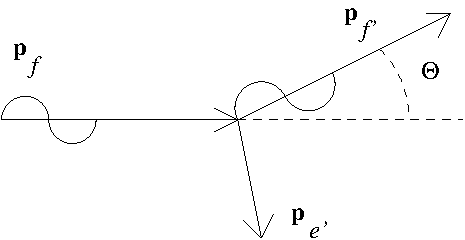
\includegraphics[scale=0.75]{compton_scattering}

\caption{Compton verstrooiing}
\end{figure}


De wet van behoud van impuls is in dit geval te schrijven als:

\begin{equation}
\mathbf{p}_{f}=\mathbf{p}_{f'}+\mathbf{p}_{e'}
\end{equation}


Door de vectoren te verschuiven, kunnen we een driehoek maken waarvoor
de cosinusregel geldt:

\begin{equation} \label{eq:cosinus}
p_{e'}^{2}=p_{f}^{2}+p_{f'}^{2}-2p_{f}p_{f'}\cos\left(\theta\right)
\end{equation}


Verder geldt de wet van behoudt van energie:

\begin{equation}
E_{f}+E_{e}=E_{f'}+E_{e'}\Longleftrightarrow
\end{equation}


Met \ref{eq:rest} en \ref{eq:foton}:

\begin{equation}
h\nu_{f}+m_{e}c^{2}=h\nu_{f'}+\sqrt{p_{e'}^{2}c^{2}+m_{e}^{2}c^{4}}\Longleftrightarrow
\end{equation}


\begin{equation}
h\nu_{f}-h\nu_{f'}+m_{e}c^{2}=\sqrt{p_{e'}^{2}c^{2}+m_{e}^{2}c^{4}}\Longleftrightarrow
\end{equation}


Kwadrateren geeft:

\begin{equation}
\left(h\nu_{f}-h\nu_{f'}+m_{e}c^{2}\right)^{2}=p_{e'}^{2}c^{2}+m_{e}^{2}c^{4}\Longleftrightarrow
\end{equation}


\begin{equation}
\left(h\nu_{f}-h\nu_{f'}\right)^{2}+2m_{e}c^{2}\left(h\nu_{f}-h\nu_{f'}\right)+m_{e}^{2}c^{4}=p_{e'}^{2}c^{2}+m_{e}^{2}c^{4}\Longleftrightarrow
\end{equation}


\begin{equation}
h^{2}\nu_{f}^{2}-2h^{2}\nu_{f}\nu_{f'}+h^{2}\nu_{f'}^{2}+2m_{e}c^{2}\left(h\nu_{f}-h\nu_{f'}\right)=p_{e'}^{2}c^{2}\Longleftrightarrow
\end{equation}


\begin{equation} \label{eq:afleiding}
\frac{h^{2}\nu_{f}^{2}}{c^{2}}-\frac{2h^{2}\nu_{f}\nu_{f'}}{c^{2}}+\frac{h^{2}\nu_{f'}^{2}}{c^{2}}+2m_{e}c\left(\frac{h\nu_{f}}{c}-\frac{h\nu_{f'}}{c}\right)=p_{e'}^{2}
\end{equation}


We kunnen nu formule \ref{eq:cosinus} aan formule \ref{eq:afleiding} koppelen:

\begin{equation}
\frac{h^{2}\nu_{f}^{2}}{c^{2}}-\frac{2h^{2}\nu_{f}\nu_{f'}}{c^{2}}+\frac{h^{2}\nu_{f'}^{2}}{c^{2}}+2m_{e}c\left(\frac{h\nu_{f}}{c}-\frac{h\nu_{f'}}{c}\right)=p_{f}^{2}+p_{f'}^{2}-2p_{f}p_{f'}\cos\left(\theta\right)\Longrightarrow
\end{equation}


\begin{equation}
-\frac{2h^{2}\nu_{f}\nu_{f'}}{c^{2}}+2m_{e}c\left(\frac{h\nu_{f}}{c}-\frac{h\nu_{f'}}{c}\right)=-\frac{2h^{2}\nu_{f}\nu_{f'}}{c^{2}}\cos\left(\theta\right)\Longleftrightarrow
\end{equation}


\begin{equation}
2m_{e}c\left(\frac{h\nu_{f}}{c}-\frac{h\nu_{f'}}{c}\right)=\frac{2h^{2}\nu_{f}\nu_{f'}}{c^{2}}\left(1-\cos\left(\theta\right)\right)\Longleftrightarrow
\end{equation}


\begin{equation}
\frac{m_{e}c}{h}\left(\frac{\nu_{f}}{c}-\frac{\nu_{f'}}{c}\right)=\frac{\nu_{f}\nu_{f'}}{c^{2}}\left(1-\cos\left(\theta\right)\right)\Longleftrightarrow
\end{equation}


\begin{equation}
\frac{m_{e}c}{h}\left(\frac{c}{\nu_{f'}}-\frac{c}{\nu_{f}}\right)=\left(1-\cos\left(\theta\right)\right)\Longleftrightarrow
\end{equation}


\begin{equation}
\left(\frac{c}{\nu_{f'}}-\frac{c}{\nu_{f}}\right)=\frac{h}{m_{e}c}\left(1-\cos\left(\theta\right)\right)\Longrightarrow
\end{equation}


\begin{equation}
\Delta\lambda=\frac{h}{m_{e}c}\left(1-\cos\left(\theta\right)\right)
\end{equation}


Deze formule geeft de verstrooiing van fotonen aan electronen. De
constante $\frac{h}{m_{e}c}$ staat ook bekend als de Compton golflengte
van een electron.

Het is natuurlijk zo dat de fotonen verstrooid worden door botsing
met de electronen. De electronen verplaatsen dus ook. Hierdoor kunnen
verschillende verschijnselen ontstaan. In een verzadigde damp kan
dit bijvoorbeeld leidden tot condensatie. Dit werd voor het eerst
waargenomen door Charles Thomas Rees Wilson toen hij een experiment
voor de vorming van wolken in een laboratorium uitvoerde. In feite
werden de condenssporen in dit geval niet door fotonen gevormd, maar
op vergelijkbare wijze door cosmische deeltjes. Een dergelijke opstelling
wordt nog steeds gebruikt en wordt een nevelkamer genoemd. Uiteraard
kunnen we ook naar de verdamping van een vloeistof kijken, een dergelijke
ruimte staat bekend als een bellenkamer. 

\end{document}
